\section{Experimental Validation}

In an attempt to show that the model works, I created the program

\begin{figure}[H]
    \centering
    % \includegraphics[width=0.45\textwidth]{assets/images/iphone_image}
    \caption{Photograph 1. The photo editing software \emph{GIMP} was used for edge detection, and the coordinates of the calibration points were selected manually. }
\end{figure}



\begin{figure}[H]
    \centering
    % 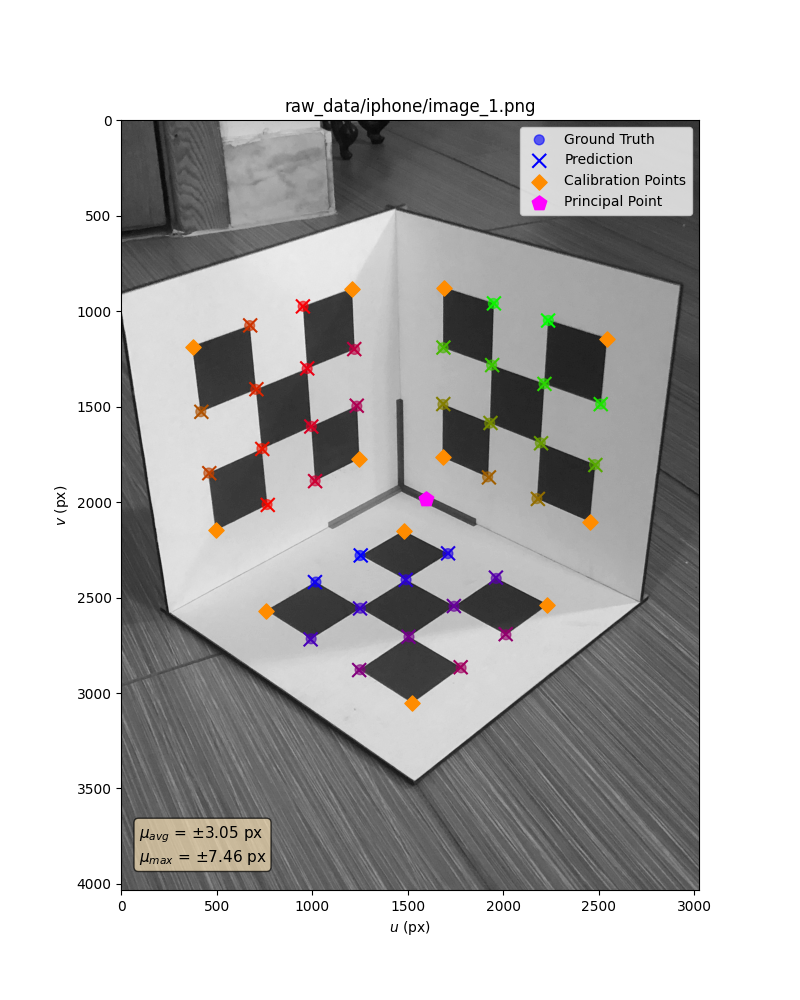
\includegraphics[width=0.6\textwidth]{assets/graphs/iphone_graph}
    \caption{Graph produced by \texttt{Matplotlib} which displays the results of the trial}
\end{figure}

\begin{equation*}
    P =
    \begin{bmatrix}
        \num{-2.5844e-03} & \num{1.7334e-03}  & \num{-4.6719e-04} & \num{6.0581e-01} \\
        \num{4.8240e-04}  & \num{4.4097e-04}  & \num{-3.1337e-03} & \num{7.9559e-01} \\
        \num{-3.3990e-07} & \num{-3.1311e-07} & \num{-2.8179e-07} & \num{4.1340e-04}
    \end{bmatrix}
\end{equation*}

\begin{table}
    \resizebox{\columnwidth}{!}{
    \begin{tabular}{p{3cm}ccccccc}
        \toprule
                                                         &             & \multicolumn{2}{c}{\textbf{\small CANON D80}} & \multicolumn{2}{c}{\textbf{\small IPHONE X}} & \multicolumn{2}{c}{\textbf{\small NIKON D100}}                                                                               \\
        \cmidrule(lr){3-4}
        \cmidrule(lr){5-6}
        \cmidrule(lr){7-8}
                                                         &             & Spreaded Out                                  & Concentrated                                 & Spreaded Out                                   & Concentrated            & Spreaded Out            & Concentrated            \\
        \midrule
        \addlinespace
        \multirow{2}{*}{\footnotesize Focal Lengths}     & $f_x$       & $\qty{8404.1}{\pixel}$                        & $\qty{8305.9}{\pixel}$                       & $\qty{3281.5}{\pixel}$                         & $\qty{3125.7}{\pixel}$  & $\qty{8144.4}{\pixel}$  & $\qty{7716.4}{\pixel}$  \\
                                                         & $f_y$       & $\qty{8387.9}{\pixel}$                        & $\qty{8338.1}{\pixel}$                       & $\qty{3279.9}{\pixel}$                         & $\qty{3137.8}{\pixel}$  & $\qty{8142.6}{\pixel}$  & $\qty{7755.5}{\pixel}$  \\
        \addlinespace
        \multirow{2}{*}{\footnotesize Principal Point}   & $c_x$       & $\qty{3151.6}{\pixel}$                        & $\qty{3400.0}{\pixel}$                       & $\qty{2043.0}{\pixel}$                         & $\qty{2031.4}{\pixel}$  & $\qty{1541.8}{\pixel}$  & $\qty{1851.5}{\pixel}$  \\
                                                         & $c_y$       & $\qty{1972.8}{\pixel}$                        & $\qty{2075.8}{\pixel}$                       & $\qty{1453.1}{\pixel}$                         & $\qty{1467.4}{\pixel}$  & $\qty{1027.9}{\pixel}$  & $\qty{1205.4}{\pixel}$  \\
        \addlinespace
        \midrule
        \addlinespace
        \multirow{3}{*}{\footnotesize Tait-Bryan Angles} & $\alpha$    & $\qty{-81.86}{\degree}$                       & $\qty{-80.32}{\degree}$                      & $\qty{-60.21}{\degree}$                        & $\qty{-60.02}{\degree}$ & $\qty{-70.83}{\degree}$ & $\qty{-67.83}{\degree}$ \\
                                                         & $\beta$     & $\qty{44.27}{\degree}$                        & $\qty{46.00}{\degree}$                       & $\qty{38.72}{\degree}$                         & $\qty{38.28}{\degree}$  & $\qty{46.44}{\degree}$  & $\qty{48.43}{\degree}$  \\
                                                         & $\gamma$    & $\qty{4.97}{\degree}$                         & $\qty{5.98}{\degree}$                        & $\qty{21.64}{\degree}$                         & $\qty{21.81}{\degree}$  & $\qty{13.89}{\degree}$  & $\qty{16.04}{\degree}$  \\
        \addlinespace
        \multirow{3}{*}{\footnotesize Translation}       & $t_x$       & $\qty{494.8}{\mm}$                            & $\qty{492.9}{\mm}$                           & $\qty{329.0}{\mm}$                             & $\qty{317.4}{\mm}$      & $\qty{840.3}{\mm}$      & $\qty{801.1}{\mm}$      \\
                                                         & $t_y$       & $\qty{537.6}{\mm}$                            & $\qty{533.5}{\mm}$                           & $\qty{321.4}{\mm}$                             & $\qty{310.2}{\mm}$      & $\qty{766.0}{\mm}$      & $\qty{726.7}{\mm}$      \\
                                                         & $t_z$       & $\qty{128.3}{\mm}$                            & $\qty{130.5}{\mm}$                           & $\qty{208.6}{\mm}$                             & $\qty{202.1}{\mm}$      & $\qty{317.2}{\mm}$      & $\qty{306.8}{\mm}$      \\
        \addlinespace
        \midrule
        \addlinespace
        \multirow{2}{*}{\footnotesize Reproj. Errors}    & $\mu_{max}$ & $\qty{11.08}{\pixel}$                         & $\qty{17.21}{\pixel}$                        & $\qty{5.58}{\pixel}$                           & $\qty{19.48}{\pixel}$   & $\qty{11.70}{\pixel}$   & $\qty{14.13}{\pixel}$   \\
                                                         & $\mu_{avg}$ & $\qty{3.56}{\pixel}$                          & $\qty{7.36}{\pixel}$                         & $\qty{2.55}{\pixel}$                           & $\qty{4.86}{\pixel}$    & $\qty{2.81}{\pixel}$    & $\qty{5.04}{\pixel}$    \\
        \addlinespace
        \bottomrule
    \end{tabular}
}


 
    \caption{Intrinsic and Extrinsic Parameters calculated by \texttt{calicam}.}
\end{table}


